\documentclass[a4paper, 10pt]{article}
\usepackage[left=2.5cm,top=3cm,right=2.5cm,bottom=2.5cm]{geometry}


\usepackage[utf8]{inputenc}
\usepackage{ragged2e}  
\usepackage{cancel}
\usepackage{mathrsfs}
\usepackage{amsmath}
\usepackage{graphicx}
\usepackage{array}
\usepackage{hyperref}
% \usepackage[spanish]{babel}
\usepackage{multicol}
\usepackage{amssymb}
\usepackage[usenames,dvipsnames,svgnames,table]{xcolor}
\usepackage{dsfont}
\usepackage{parskip}

\begin{document}
	\section{RESULTADOS}
	 Se tuvieron las siguientes observaciones como parte del armado del sistema experimental:
	 \begin{itemize}
	 	\item  La longitud de la cuerda (sin tensarla) era de $ (331.5\pm 0.05) cm $
	 	\item La masa de la cuerda era de $( 3.6 \pm 0.05)g $
	 	\item La densidad de masa de la cuerda resultó entonces de (véase apéndice) 
	 	$$\mu=\left(0.0108\pm0.0001\right)\dfrac{g}{cm}=(0.00108\pm 0.00001)\dfrac{kg}{m}$$
	 	\item La longitud de la cuerda tensada (desde el generador de ondas hasta el punto de unión con la polea) fue de $ (267 \pm 0.05) cm $
	 \end{itemize}
 
 	Luego, para obtener la medición de la longitud de la onda estacionaria producida por el generador, con dos valores de masa distintos pero con el mismo armónico ($n=4$), se obtuvieron los siguientes resultados 
 	 	
	\begin{table}[ht]
	\centering
	\caption{Resultados obtenidos de las mediciones.}
	 	\begin{tabular}{|l|c|c|}
		 		\hline
		 		Dato Experimental & Experimento 1 & Experimento 2 \\
		 		\hline
		 		Masa del portapesas & $ 0.005 kg $ & $ 0.005 kg $ \\
		 		\hline
		 		Masa agregada $ m $& $ 0.150 kg $ & $ 0.200 kg $  \\
		 		\hline
		 		Masa total $ M $ & $ 0.155kg $ & $ 0.205kg $  \\
		 		\hline
		 		Tensión en la cuerda $ T $ & $ 1.52055 Nw $  & $ 2.0110 Nw$ \\
		 		\hline
		 		Valor de la frecuencia $ f $ & $ (29\pm 0.05)Hz$  & $ (33.7\pm 0.05)Hz $ \\
		 		\hline
		 		Longitud de onda $ \lambda $ & $ (134\pm0.05)cm $ & $ (131\pm0.05)cm $  \\
		 		\hline
	 	\end{tabular}
 	\end{table}
 
 	Para los cálculos de la velocidad con las fórmulas $ (1) $ y $ (2) $ de la práctica, los resultados fueron los siguientes
 	
 	\begin{table}[ht]
 	\footnotesize
 	\centering
 	\caption{Cálculo de la velocidad de onda.}
 		\begin{tabular}{|c|c|c|c|c|c|c|c|}
	 		\hline
	 		Experi-& $ \lambda $ $ (cm)$ & $ f $ $ (Hz)$ & $ v_a=\lambda\cdot f $ & $ T $ & $ \mu  (\frac{kg}{m})$ & $ v_b=\sqrt{\frac{T}{\mu}} $ & Diferencia \\
	 		mento & $ \pm 0.05cm $ & $ \pm 0.05 Hz $ & $ (\frac{cm}{s}) $ & $ (Nw) $ & $ \pm 0.00001\frac{kg}{m} $ & $ (\frac{cm}{s}) $ & $ |v_a-v_b| (\frac{cm}{s}) $ \\
	 		\hline
	 		1 & 134 & 29 & $ 3886\pm8.15 $ & 1.52055 & $0.00108$ & $ 3741.889\pm 26.26753 $ & $ 144.111 $ \\
	 		\hline
	 		2 & 131 & 33.7 & $ 4414.7\pm8.235 $ & 2.0110 & $0.00108$ & $ 4303.303\pm 34.74093 $ & $ 111.397 $ \\
	 		\hline
	 	\end{tabular}
 	\end{table} 
  	
	Luego, para una masa fija de $ 155g $, se obtuvo que la frecuencia del armónico fundamental ($ n=1 $) era de $$f_1=(7\pm0.05)Hz$$
	
	Tomando este valor como \textit{teórico} (sin la incertidumbre) y empleando la fórmula ( $f_n=nf_1$ no sé que \#), los resultados fueron los siguientes
	
	\begin{table}[ht]
		\centering
		\caption{Frecuencia en los modos de oscilación.}
		\begin{tabular}{|c|c|c|c|}
		\hline
		Armónico & $ f $ teórica & $ f $ observada en $Hz$  & Error  \\
		$ n $ & en $ Hz $ & $\pm 0.05 Hz $ & relativo\\
		\hline
		2 & 14 & 15 & $ 7.1428\% $ \\
		\hline
		3 & 21 & 22 & $ 4.7619\% $ \\
		\hline
		4 & 28 & 29 & $ 3.5714\% $ \\
		\hline
		\end{tabular}
	\end{table}
	
	Para la siguiente parte del experimento, se optó por dejar una frecuencia fija de $f=(22\pm 0.05) Hz$, y haciendo variar la masa del portapesas para obtener distintos armónicos, los resultados para la tensión en la cuerda son los siguientes
	
	\begin{table}[ht]
		\centering
		\caption{Tensión en la cuerda para distintas masas con misma frecuencia.}
		\begin{tabular}{|c|c|c|}
			\hline
			Armónico& Masa & Tensión \\
			$ n $& $ m $ ($ kg $) & $ T $ ($ Nw $)  \\
			\hline
			3& 0.155 & 1.52055 \\
			\hline
			4& 0.105 & 1.03005  \\
			\hline
			5& 0.055 & 0.53955  \\
			\hline
			6& 0.025 & 0.24525  \\
			\hline
		\end{tabular}
	\end{table}
 	
 	Luego, se realizaron las gráficas de $ T $ vs. $ n $ y $ T $ vs. $ 1/n^2 $, donde $ n $ representa el número de armónico. Tales gráficas se muestran a continuación.

 	\begin{figure}[ht]
 		\centering
 		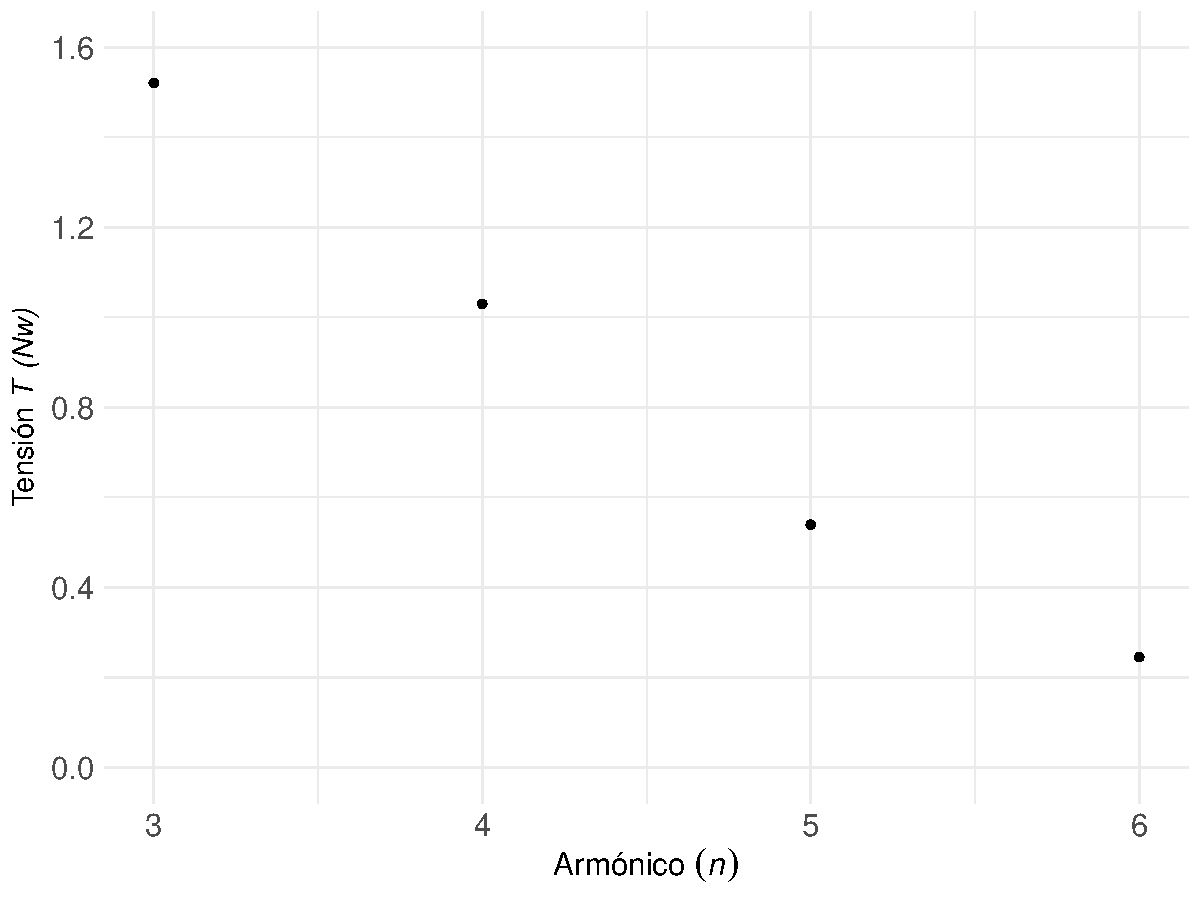
\includegraphics[width= 1\linewidth]{T vs n.pdf}
 		\caption{$T$ vs. \(n\).}
 		\label{fig:graf1}
 	\end{figure}
 
 	\begin{figure}[ht]
 		\centering
 		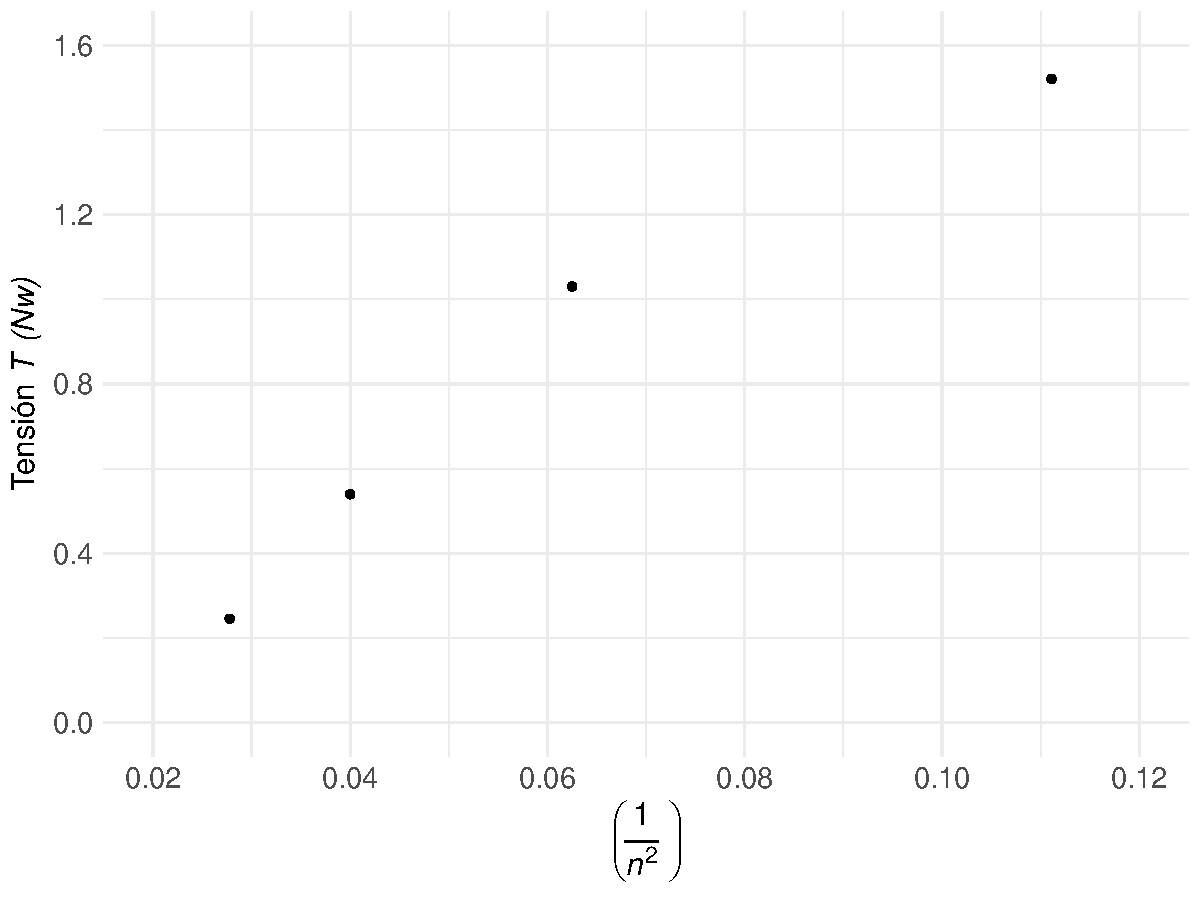
\includegraphics[width= 1\linewidth]{T vs n2.pdf}
 		\caption{$T$ vs. $ \left(\dfrac{1}{n^2}\right) $.}
 		\label{fig:graf2}
 	\end{figure}
 	\newpage
 	A partir de esta última relación, se obtuvo la estimación de la recta por mínimos cuadrados que se aproximara a estas observaciones, resultando que
 	$$ T=[(14.90009\pm 2.29002) Nw]\left(\dfrac{1}{n^2}\right)-(0.06533\pm 0.15625) Nw $$ 
 	
 	La gráfica entonces queda de la siguiente forma
 	
 	\begin{figure}[ht]
 		\centering
 		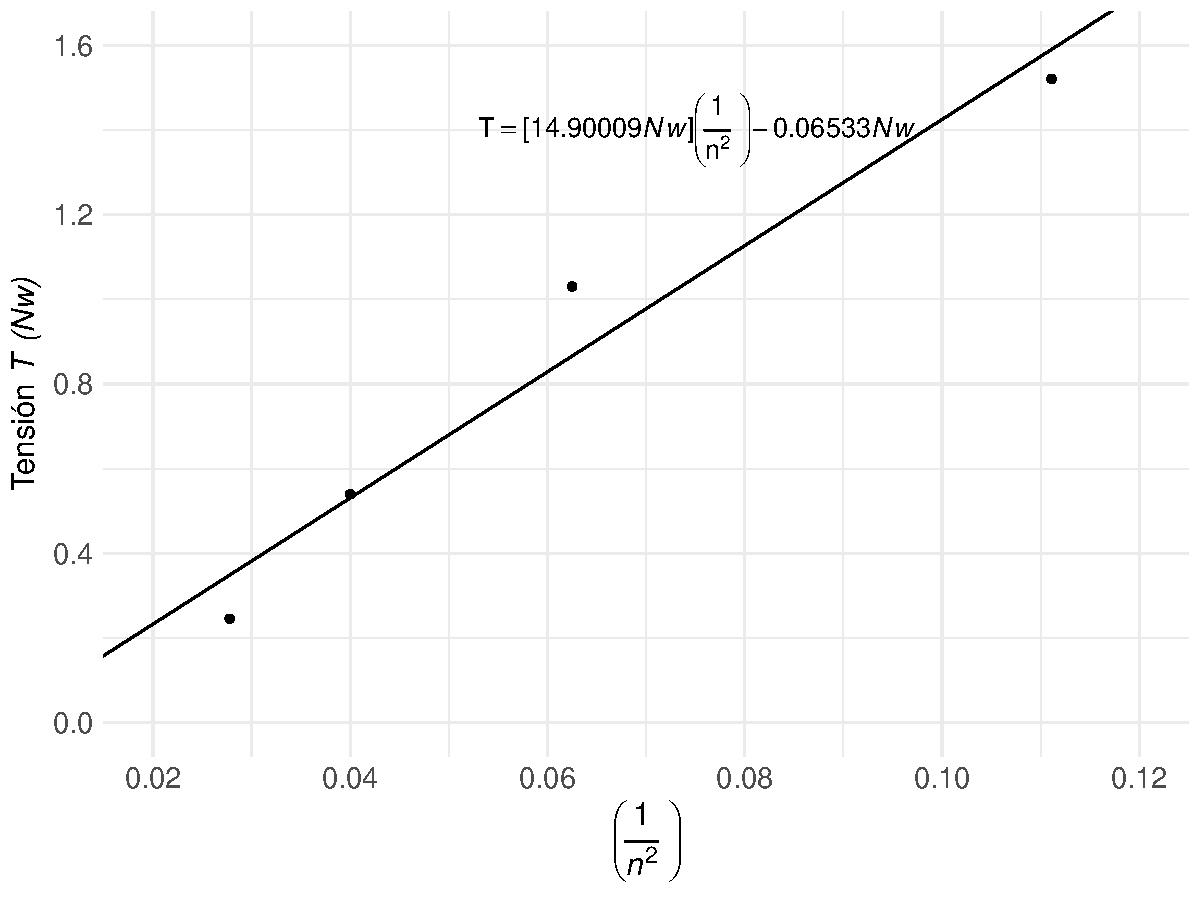
\includegraphics[width= 1\linewidth]{T vs n2 2.pdf}
 		\caption{Estimación por mínimos cuadrados.}
 		\label{fig:graf3}
 	\end{figure}
 	\newpage
 	Luego, a partir del valor de la estimación de la pendiente, así como de la fórmula 
 	$$T=\left(4\mu f^2 L^2\right)\left(\dfrac{1}{n^2}\right)$$
 	
 	se puede hacer una estimación para la densidad de masa lineal de la cuerda empleada. Haciendo la estimación de $ \mu $ a partir de esto (véase el apéndice para los cálculos), se obtuvo que 
 	$$\mu=(0.00107\pm0.0001)\dfrac{kg}{m}$$
 	
 	Comparando este valor con el obtenido al inicio de los resultados, se tiene tan solo una diferencia de 
 	$$|0.00108-0.00107|\dfrac{kg}{m}=0.00001\dfrac{kg}{m}$$
	\newpage
	
	\section{APÉNDICE.}
	
	\subsection{--- Propagación de la Incertidumbre ---}
	
	La propagación de la incertidumbre para la suma, el producto y un cociente están dadas (respectivamente) por
	\begin{align*}
		(x\pm \delta x)\pm(y\pm \delta y)&=(x\pm y)\pm(\delta x+\delta y)\\\\
		(x\pm\delta x)(y\pm\delta y)&=x\cdot y\pm\left(|y|\delta x+|x|\delta y \right)\\\\
		\dfrac{x\pm\delta x}{y\pm\delta y}&=\dfrac{x}{y}\pm\left(\dfrac{\delta x}{|y|}+|x|\dfrac{\delta y}{|y|^2}\right)
	\end{align*}
	
	\subsection{--- Incertidumbre en $ \sqrt{\cdot} $ ---}
	
	Consúltese [] para la deducción de la ecuación (\ref{eq:prop_inc}). Si $f$ es una función de $\mathbb{R}^n$ a $\mathbb{R}$ en la cual se le pueden medir sus variables (cada una asociada con su respectiva incertidumbre)
	$$f(x_1\pm\Delta x_1,x_2\pm\Delta x_2,...,x_n\pm\Delta x_n)$$
	entonces (si la función es derivable) la propagación de la incertidumbre está dada por
	\begin{equation}
		\Delta f=\pm\left(\displaystyle\sum_{i=1}^k\Delta x_i\cdot\left|\dfrac{\partial f(x_i)}{\partial x_i}\right| \right)
		\label{eq:prop_inc}
	\end{equation} 
	
	Para el caso de la función $ \sqrt{\cdot} $, se tiene que 
	\begin{align*}
		\sqrt{x\pm\Delta x}&=
		\sqrt{x}\pm\left(\Delta x\cdot\left|\dfrac{d(x^{\frac{1}{2}})}{dx}\right|\right)=\\\\
		&=\sqrt{x}\pm\left(\Delta x\cdot\dfrac{1}{2\sqrt{x}}\right)
	\end{align*} 
	
	Por lo que
	\begin{equation}
		\sqrt{x\pm\Delta x}=\sqrt{x}\pm\dfrac{\Delta x}{2\sqrt{x}}
		\label{rc}
	\end{equation}
	
	\subsection{--- Densidad de Masa Lineal $ \mu $ ---}
	
	Para el cálculo de la densidad de masa lineal, se tiene
	\begin{align*}
		\dfrac{(3.6 \pm 0.05)g}{(331.5\pm 0.05) cm }&=\left[\dfrac{3.6}{331.5}\pm \left(\dfrac{0.05}{331.5}+3.6\cdot \dfrac{0.05}{331.5^2}\right)\right]\dfrac{g}{cm}=\\\\
		&=\left(0.0108\pm0.0001\right)\dfrac{g}{cm}=\\\\
		&=\left[\left(0.0108\pm0.0001\right)\dfrac{g}{cm}\right]\cdot
		\left(\dfrac{1kg}{1000 g}\right)\cdot\left(\dfrac{100 cm}{1 m}\right)=\\\\
		&=(0.00108\pm 0.00001)\dfrac{kg}{m}
	\end{align*}
	
	
	\subsection{--- Cálculo de la Tensión y Velocida ---}
	
	Para el cálculo de la tensión en la cuerda a partir de la masa agregada en el portapesas, del diagrama de cuerpo libre (ver figura no sé), se tiene que $$ T-w=0\Longrightarrow T=w=m\cdot g$$
	
 	Para el primer sistema, la masa total fue de $ 155 g=0.155 kg $. Por ende, la tensión en la cuerda era de 
 	$$T_1=(0.155 kg)\cdot \left(9.81\frac{m}{s^2}\right)=1.5205 Nw$$
 	
 	Con este valor, y con los datos experimentales obtenidos, se obtuvo lo siguiente
 	\begin{align*}
 		v_a=\lambda\cdot f&=[(134\pm0.05)cm]\cdot[(29\pm 0.05)Hz]=\\
 		&=[(134\cdot29)\pm(134\cdot0.05+ 29\cdot0.05)]\left(\dfrac{cm}{s}\right)=\\
 		&=(3886\pm8.15)\dfrac{cm}{s}
 	\end{align*}
 	Por otro lado, como
 	\begin{align*}
 		\dfrac{T_1}{\mu}&=\dfrac{1.52055 Nw}{(0.00108\pm 0.00001)\dfrac{kg}{m}}=\\\\
 		&=\left[\dfrac{1.52055}{0.00108}\pm\left(1.52055\cdot\dfrac{0.00001}{0.00108^2}\right)\right]\left(\dfrac{\dfrac{kg\cdot m}{s^2}}{\dfrac{kg}{m}}\right)=\\\\
 		&=(1400.173\pm19.65804)\dfrac{m^2}{s^2}
 	\end{align*}
 	
 	Haciendo uso de (\ref{rc}), resulta que
 	\begin{align*}
 		v_b&=\sqrt{\dfrac{T}{\mu}}=\sqrt{(1400.173\pm19.65804)\dfrac{m^2}{s^2}}\\\\
 		&=\left(\sqrt{1400.173}\pm\dfrac{19.65804}{2\cdot\sqrt{1400.173}}\right)\dfrac{m}{s}=\\\\
 		&=(37.41889\pm 0.26267)\dfrac{m}{s}=\\\\
 		&=(3741.889\pm 26.26753)\dfrac{cm}{s}
 	\end{align*}
 
 	Así pues
 	\begin{center}
 		\begin{multicols}{2}
	 		$ v_a=(3886\pm8.15)\dfrac{cm}{s} $\\
	 		$ v_b=(3741.889\pm 26.26753)\dfrac{cm}{s} $
	 	\end{multicols}
 	\end{center}
 	
 	$$\therefore |v_a-v_b|=\left|3886-3741.889\right|\frac{cm}{s}=144.111\frac{cm}{s}$$
 	
 	Similarmente, para el segundo sistema, la masa total fue de $ 205g=0.205kg $, por lo que la tensión de la cuerda resulta de
 	$$T_2=(0.205 kg)\cdot \left(9.81\frac{m}{s^2}\right)=2.01105 Nw$$ 
 	y con los datos experimentales, se tiene que
 	
 	\begin{align*}
 		v_a=\lambda\cdot f&=[(131\pm0.05)cm]\cdot[(33.7\pm 0.05)Hz]=\\
 		&=[(131\cdot33.7)\pm(131\cdot0.05+ 33.7\cdot0.05)]\left(\dfrac{cm}{s}\right)=\\
 		&=(4414.7\pm8.235)\dfrac{cm}{s}
 	\end{align*}
 	Por otro lado
 	\begin{align*}
 		\dfrac{T_2}{\mu}&=\dfrac{2.01105 Nw}{(0.00108\pm 0.00001)\dfrac{kg}{m}}=\\\\
 		&=\left[\dfrac{2.01105}{0.00108}\pm\left(2.01105\cdot\dfrac{0.00001}{0.00108^2}\right)\right]\left(\dfrac{\dfrac{kg\cdot m}{s^2}}{\dfrac{kg}{m}}\right)=\\\\
 		&=(1851.842\pm25.99934)\dfrac{m^2}{s^2}
 	\end{align*}
 	
 	Nuevamente haciendo uso de (\ref{rc}), se obtiene que
 	\begin{align*}
 		v_b&=\sqrt{\dfrac{T}{\mu}}=\sqrt{(1851.842\pm25.99934)\dfrac{m^2}{s^2}}\\\\
 		&=\left(\sqrt{1851.842}\pm\dfrac{25.99934}{2\cdot\sqrt{1851.842}}\right)\dfrac{m}{s}=\\\\
 		&=(43.03303\pm 0.34740)\dfrac{m}{s}=\\\\
 		&=(4303.303\pm 34.74093)\dfrac{cm}{s}
 	\end{align*}
 	
 	Entonces
 	\begin{center}
 		\begin{multicols}{2}
 			$ v_a=(4414.7\pm8.235)\dfrac{cm}{s} $\\
 			$ v_b=(4303.303\pm 34.74093)\dfrac{cm}{s} $
 		\end{multicols}
 	\end{center}
 	
 	$$\therefore |v_a-v_b|=\left|4414.7-4303.303\right|\frac{cm}{s}=111.397\frac{cm}{s}$$
 	
 	\subsection{--- Nueva Estimación para $ \mu $ ---}
 	
 	A partir de la relación 
 	$$T=\left(4\mu f^2 L^2\right)\left(\dfrac{1}{n^2}\right)$$
 	se puede decir que
 	$$\mu=\dfrac{Tn^2}{4f^2L^2}$$
 	
 	Luego, de la estimación para la recta por mínimos cuadrados (calculada con el software R), se obtuvo 
 	$$ T=[(14.90009\pm 2.29002) Nw]\left(\dfrac{1}{n^2}\right)-(0.06533\pm 0.15625) Nw $$
 	
 	El valor de la pendiente $a=(14.90009\pm 2.29002) Nw$ representa el valor de $ Tn^2 $, puesto que
 	$$a=\dfrac{\Delta y}{\Delta x}=\dfrac{T}{\dfrac{1}{n^2}}=Tn^2$$ 
 	y además, de los datos experimentales se tiene que
 	\begin{itemize}
 		\item[] $f=(22\pm0.05)Hz\Longrightarrow$
 		\begin{align*}
 			f^2&=(22\pm0.05)\cdot(22\pm0.05)Hz^2\\
 			&=(22^2\pm2\cdot22\cdot0.05)\dfrac{1}{s^2}=(484\pm2.2)\dfrac{1}{s^2}
 		\end{align*}
 		 
 		
 		\item[]$L=(2.67\pm0.0005)m\Longrightarrow L^2=(2.67\pm0.0005)\cdot(2.67\pm0.0005)m^2=$\\
 		\hspace{5cm}$=(2.67^2\pm2\cdot2.67\cdot0.0005)m^2=(7.1289\pm0.00267)m^2$
 	\end{itemize}
 	
 	Entonces
 	\begin{align*}
 		4f^2L^2&=4\left[(484\pm2.2)\dfrac{1}{s^2}\right]\left[(7.1289\pm0.00267)m^2\right]\\
 		&=(1936\pm8.8)(7.1289\pm0.00267)\dfrac{m^2}{s^2}\\
 		&=[1936\cdot7.1289\pm(1936\cdot0.00267+8.8\cdot7.1289)]\dfrac{m^2}{s^2}\\
 		&=(13801.55\pm 67.90344)\dfrac{m^2}{s^2}
 	\end{align*}
 
 	Y así
 	\begin{align*}
 		\mu&=\dfrac{Tn^2}{4f^2L^2}=\dfrac{(14.90009\pm 2.29002)}{(13801.55\pm 67.90344)}\dfrac{\dfrac{kg\cdot m}{s^2}}{\dfrac{m^2}{s^2}}\\\\
 		&=\left[\dfrac{14.90009}{13801.55}\pm\left(\dfrac{2.29002}{13801.55}+14.90009\cdot\dfrac{67.90344}{13801.55^2}\right)\right]\dfrac{kg}{m}\\\\
 		&=(0.00107\pm0.0001)\dfrac{kg}{m}
 	\end{align*}
\end{document}
